\documentclass[a4paper, 16pt]{article}
\usepackage[utf8]{inputenc}
\usepackage[english, russian]{babel}
\usepackage{indentfirst}
\usepackage[left=20mm, top=20mm, right=20mm,
 bottom=20mm, head=1mm, foot=1mm]{geometry}
\usepackage{tikz}
\usepackage{amsmath, amsfonts, amssymb}
\usepackage{graphicx}
\usepackage{fancybox, fancyhdr}
\usepackage{hyperref}
\usepackage{listings}
\usepackage{caption}
\usepackage{subcaption}
\usepackage{xcolor}
\pagestyle{fancy}
\fancyhf{}
\fancyhead[L]{Лабораторная работа №3}
\fancyhead[R]{Частотные методы}
\fancyfoot[C]{\thepage}
\graphicspath{{images/}}
\usetikzlibrary{patterns}
\definecolor{LightGray}{gray}{0.95}
\lstdefinestyle{pycode}{
    language=Python,
    basicstyle=\footnotesize\ttfamily,
    numbers=left,
    numberstyle=\tiny\color{gray},
    stepnumber=1,
    numbersep=5pt,
    backgroundcolor=\color{LightGray},
    showspaces=false,
    showstringspaces=false,
    showtabs=false,
    tabsize=4,
    captionpos=b,
    breaklines=true,
    breakatwhitespace=false,
    frame=single,
    rulecolor=\color{black},
    linewidth=\linewidth,
    keywordstyle=\color{red}\bfseries,
    commentstyle=\color{green!40!black},
    stringstyle=\color{blue},
    escapeinside={\%*}{*)},
    xleftmargin=0pt,
    framexleftmargin=0pt,
    framexrightmargin=0pt
}
\lstset{style=pycode}
\hypersetup{
    colorlinks=true,
    linkcolor=blue,
    filecolor=magenta,      
    urlcolor=cyan,
    pdftitle={contents setup},
    pdfpagemode=FullScreen,
}
\allowdisplaybreaks
\DeclareMathOperator{\sinc}{sinc}
\newcommand{\frc}[2]{\raisebox{2pt}{$#1$}\big/\raisebox{-3pt}{$#2$}}

\begin{document}
\begin{titlepage}

    \begin{center}
    \vfill
    
    Федеральное государственное автономное образовательное учреждение высшего образования\\
    «Национальный Исследовательский Университет ИТМО»\ \\
    
    \vfill
    {\large\bf ЛАБОРАТОРНАЯ РАБОТА №3\\
        ПО ПРЕДМЕТУ «ЧАСТОТНЫЕ МЕТОДЫ»\\
        ПО ТЕМЕ «ЖЕСТКАЯ ФИЛЬТРАЦИЯ»}
    \vfill
        
    \begin{flushright}
        \begin{minipage}{.45\textwidth}
        {
            \hbox{Лектор: Перегудин А. А.}
            \hbox{Практик: Пашенко А. В.}
            \hbox{Студент: Румянцев А. А.}
            \hbox{Поток: ЧАСТ.МЕТ. 1.3}
            \hbox{}
            \hbox{Факультет: СУиР}
            \hbox{Группа: R3241}
        }
        \end{minipage}
    \end{flushright}
    
    \vfill
            
    Санкт-Петербург\\
    2024
    \end{center}
    \end{titlepage}
    \setlength{\parskip}{1.5mm}
    
    \tableofcontents

    \newpage
    \section{Задание 1. Жесткие фильтры.}
    Зададим такие числа $a,\,t_1,\,t_2$, что $t_1<t_2$, и рассмотрим функцию $g$ такую, что
    $g(t)=a$ при $t\in[t_1,t_2]$ и $g(t)=0$ при других $t$. $$\sqsupset a=2,\ \ t_1=-1.5,\ \ t_2=2.5,\ \ g(t)=
    \begin{cases}
        2, & t\in[t_1,t_2]\\
        0, & \text{ otherwise}
    \end{cases}
    $$


    Выберем интервал времени $T=10$ и шаг дискретизации $dt=0.1$. Зададим в python массив времени $t$ от $-\,\frc{T}{2}$ до $\frc{T}{2}+dt$
    с шагом $dt$ и включенной последней точкой. Найдем список значений $g$ и зададим зашумленную версию сигнала как
    $$
    u=g+b\cdot(\text{random}(\text{len}(t))-0.5) + c\cdot \sin(d\cdot t);
    $$


    В данном задании мы выполняем жесткую фильтрацию сигнала $u$. Алгоритм следующий: находится Фурье-образ от сигнала,
    обнуляются его значения на некоторых диапазонах частот, затем сигнал восстанавливается обратным преобразованием Фурье.
    Далее строятся графики с помощью программы на языке python. Используемый код с пояснениями находится в отдельной секции.


    В задаваемом сигнале параметр $a$ отвечает за высоту, на которую поднимется часть сигнала от нуля, а $t_1 \text{ и } t_2$ -- начало
    и конец промежутка с подъемом соответственно. Таким образом, на интервале длины $t_2-t_1=2.5+1.5=4$, начиная с $t_1=-1.5$ и заканчивая $t_2=2.5$,
    на высоте $a=2$ будет находится часть от всего сигнала, который, в свою очередь, располагается на промежутке $[-\,\frc{T}{2},\frc{T}{2}]=[-5,5]$
    длины $2\cdot \frc{T}{2}=10$. Параметры $b,\,c,\,d$ отвечают за шум, присутствующий в сигнале. Далее будут рассмотрены графики и сделаны выводы о
    влиянии каждого параметра на сам сигнал и на его результат фильтрации.


    \subsection{Убираем высокие частоты.}
    Возьмем параметр $c=0$. Далее действуем в соответствии с алгоритмом. Возьмем некоторый диапазон частот $[-v_0, v_0]$, на котором оставим Фурье-образ
    сигнала $u$ неизменным, а на остальных частотах обнулим его значения. Построим сравнительные графики исходного и фильтрованного сигналов на некотором
    интервале $[t_1,t_2]$, а также модуля Фурье-образа исходного и фильтрованного сигналов. Исследуем влияние частоты среза $v_0$ и значения параметра $b$
    на эффективность фильтрации.
    
    
    Далее будут приведены рисунки полученных графиков. На каждом графике подписаны выбранные значения $b,\,c,\,d,\,v_0$
    (хотя, при условии, что $c=0$, менять или рассматривать параметр $d$ не требуется). Также отмечена легенда -- синим цветом
    обозначается оригинальный сигнал, красным фильтрованный.
    \begin{figure}[!htb]
        \centering
        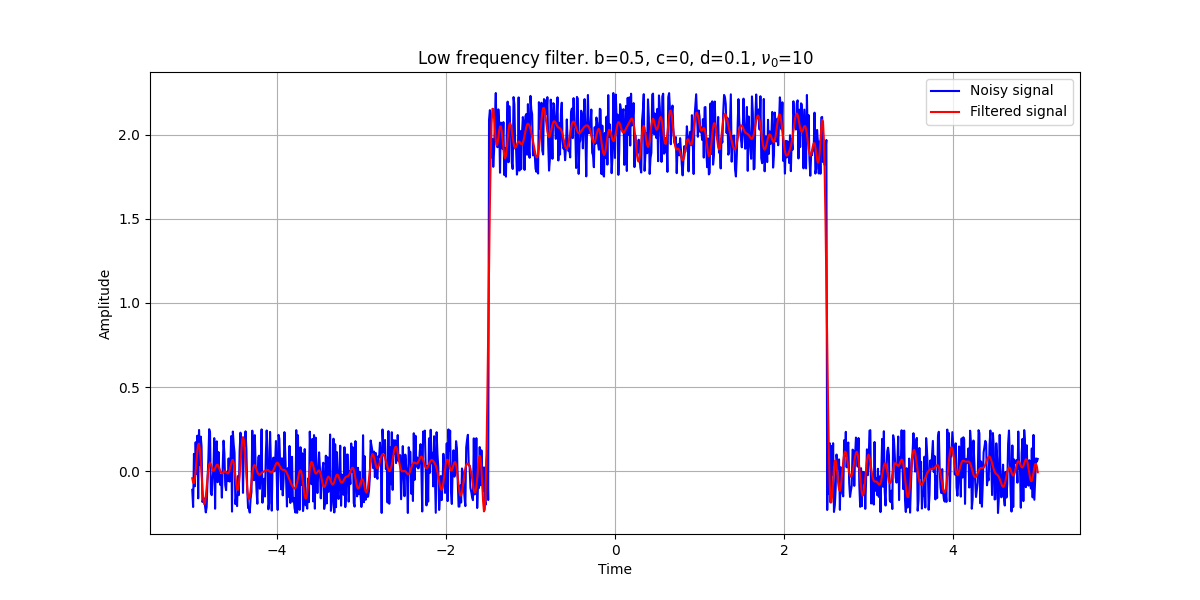
\includegraphics[scale=0.485]{1_u_flt_u_nohigh.png}
        \captionsetup{skip=0pt}
        \caption{График исходного и фильтрованного сигналов}
        \label{fig:fig1}
    \end{figure}
    \newpage
    \begin{figure}[!htb]
        \centering
        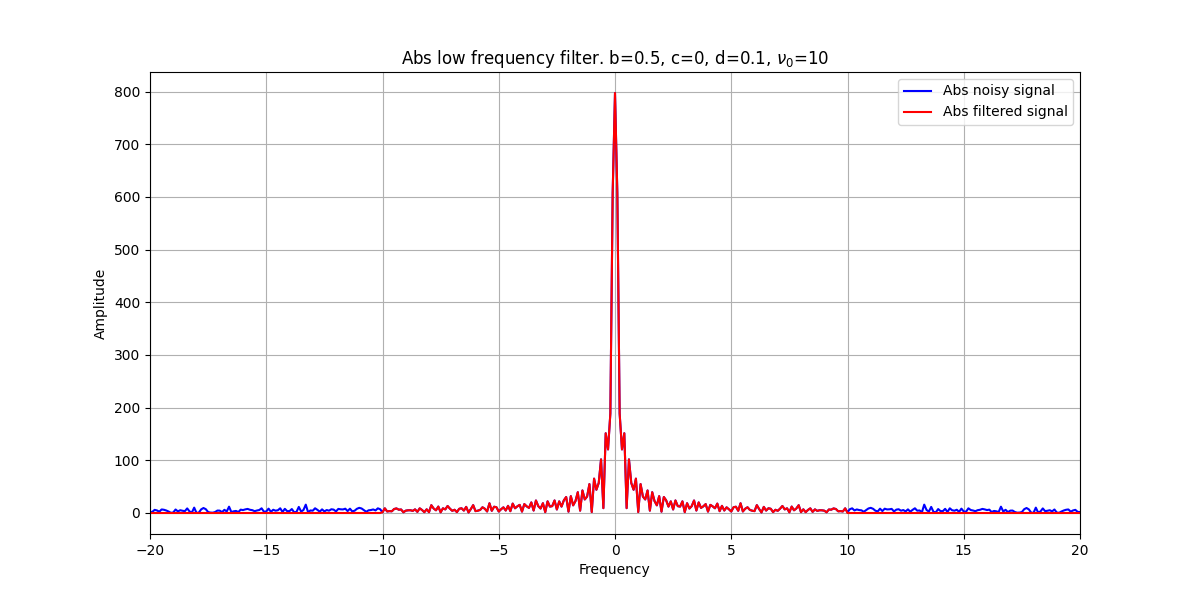
\includegraphics[scale=0.485]{1_abs_u_U_nohigh.png}
        \captionsetup{skip=0pt}
        \caption{График модуля Фурье-образа исходного и фильтрованного сигналов}
        \label{fig:fig2}
    \end{figure}
    \begin{figure}[!htb]
        \centering
        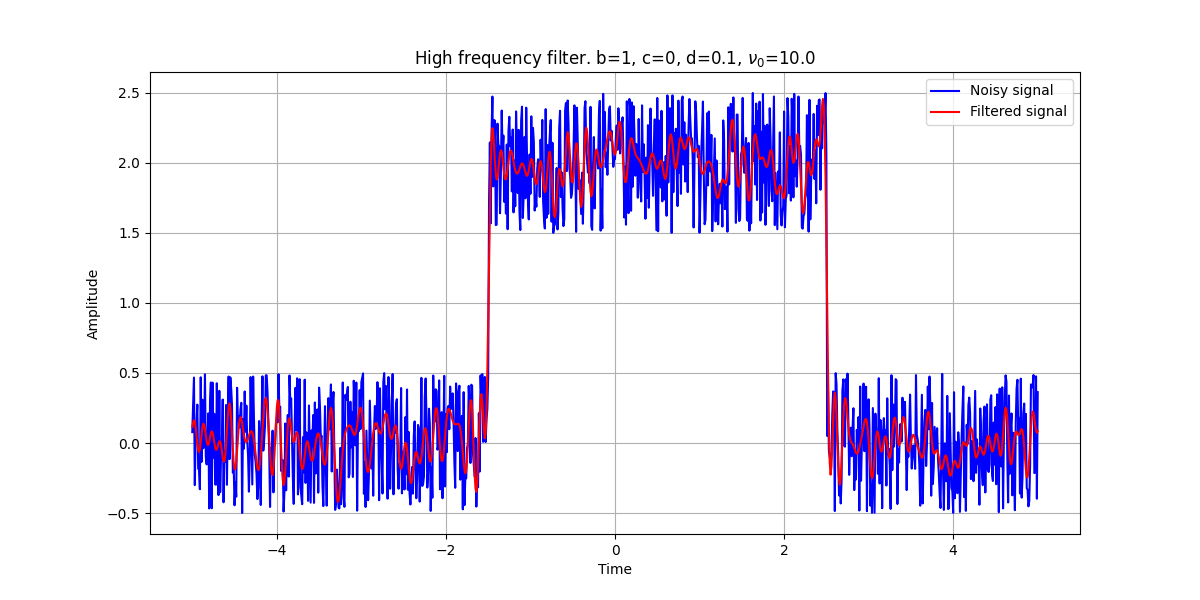
\includegraphics[scale=0.485]{2_u_flt_u_nohigh.png}
        \captionsetup{skip=0pt}
        \caption{График исходного и фильтрованного сигналов}
        \label{fig:fig3}
    \end{figure}
    \begin{figure}[!htb]
        \centering
        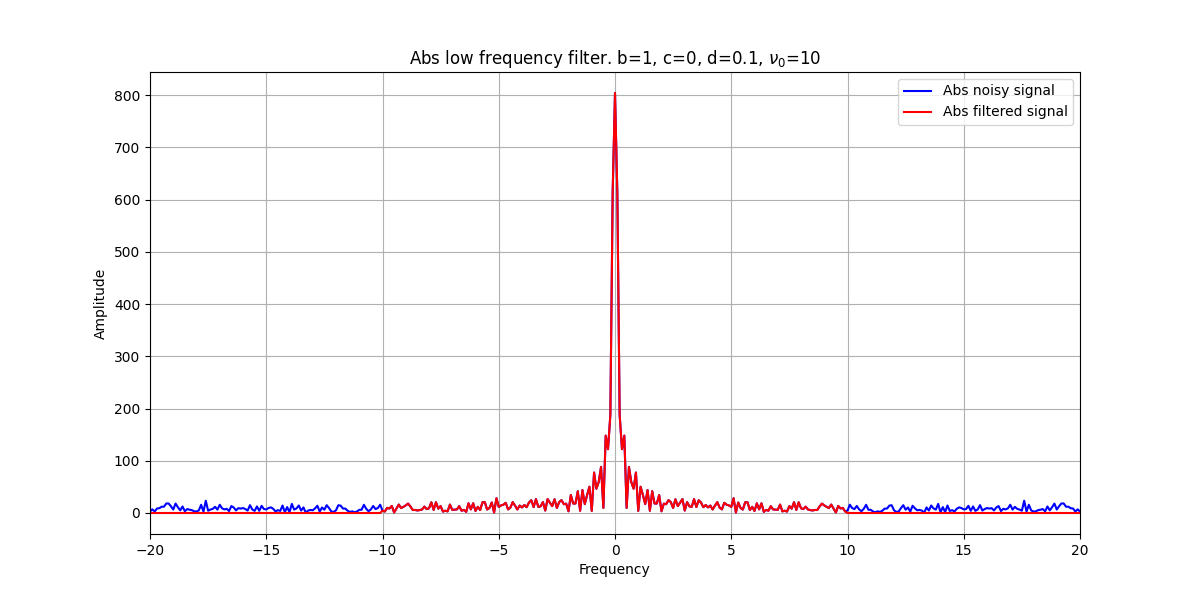
\includegraphics[scale=0.485]{2_abs_u_U_nohigh.png}
        \captionsetup{skip=0pt}
        \caption{График модуля Фурье-образа исходного и фильтрованного сигналов}
        \label{fig:fig4}
    \end{figure}
    \newpage
    \begin{figure}[!htb]
        \centering
        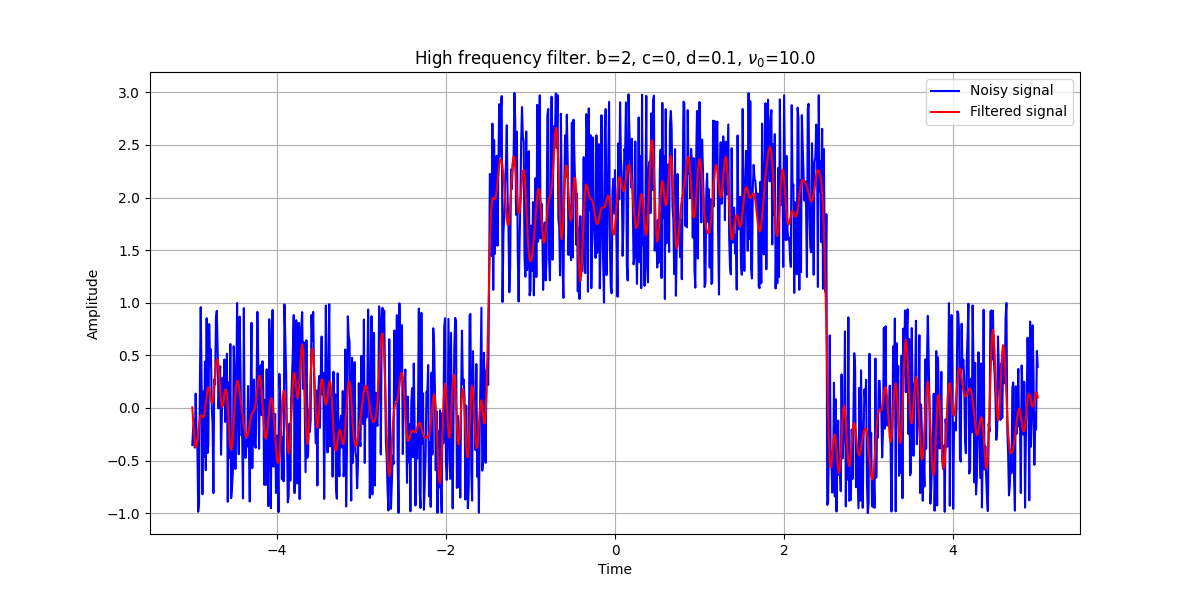
\includegraphics[scale=0.485]{3_u_flt_u_nohigh.png}
        \captionsetup{skip=0pt}
        \caption{График исходного и фильтрованного сигналов}
        \label{fig:fig5}
    \end{figure}
    \begin{figure}[!htb]
        \centering
        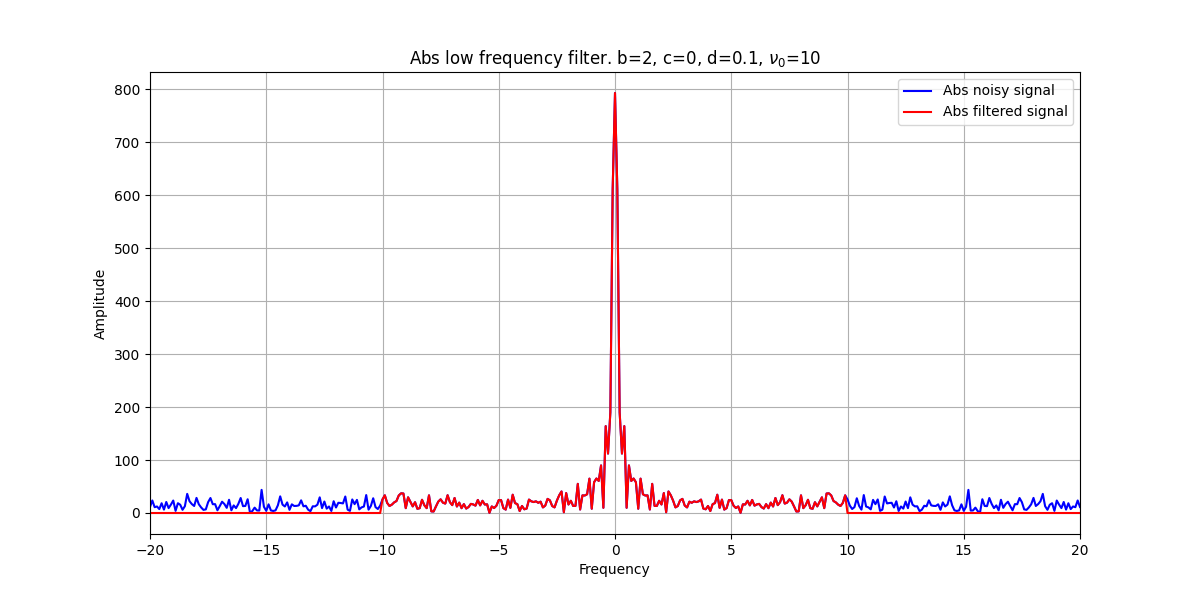
\includegraphics[scale=0.485]{3_abs_u_U_nohigh.png}
        \captionsetup{skip=0pt}
        \caption{График модуля Фурье-образа исходного и фильтрованного сигналов}
        \label{fig:fig6}
    \end{figure}
    \begin{figure}[!htb]
        \centering
        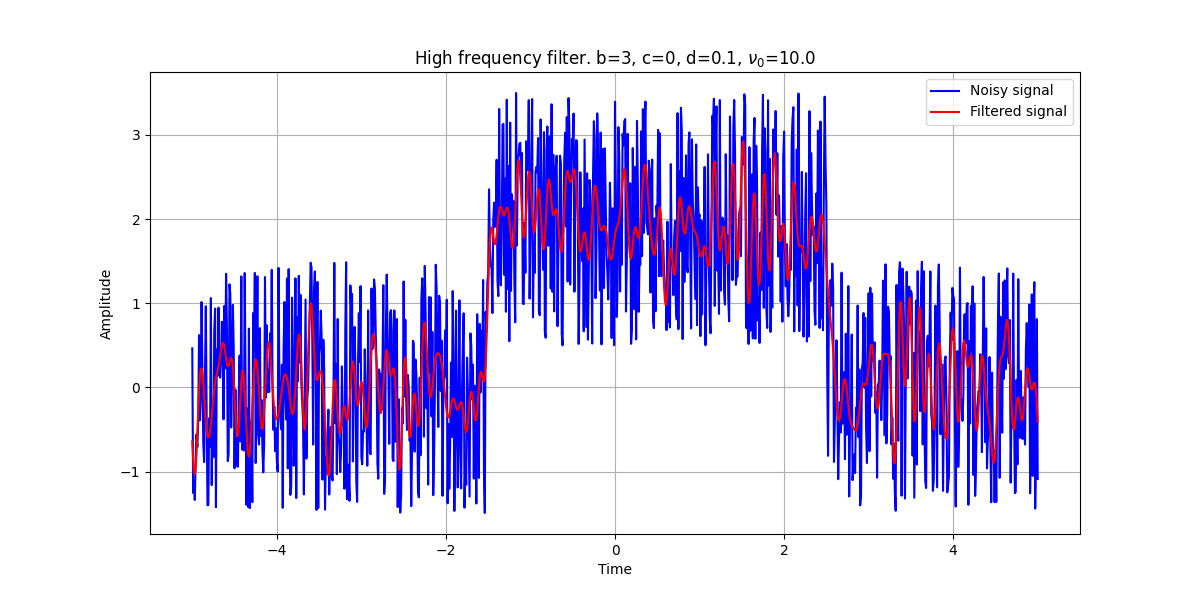
\includegraphics[scale=0.485]{5_u_flt_u_nohigh.png}
        \captionsetup{skip=0pt}
        \caption{График исходного и фильтрованного сигналов}
        \label{fig:fig7}
    \end{figure}
    \newpage
    \begin{figure}[!htb]
        \centering
        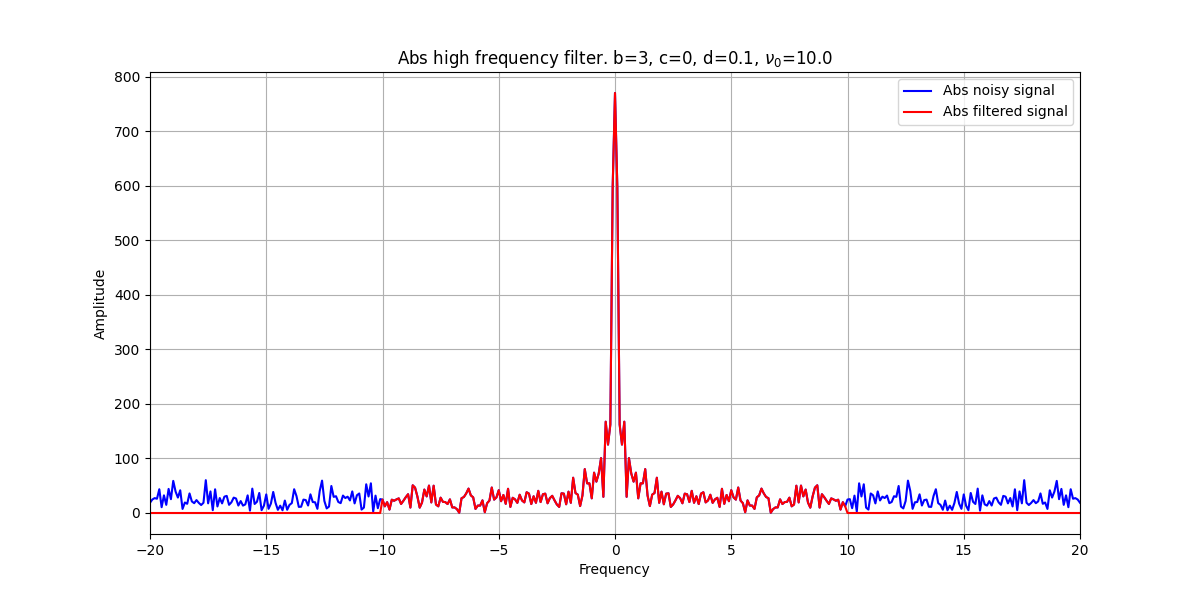
\includegraphics[scale=0.485]{5_abs_u_U_nohigh.png}
        \captionsetup{skip=0pt}
        \caption{График модуля Фурье-образа исходного и фильтрованного сигналов}
        \label{fig:fig8}
    \end{figure}
    \begin{figure}[!htb]
        \centering
        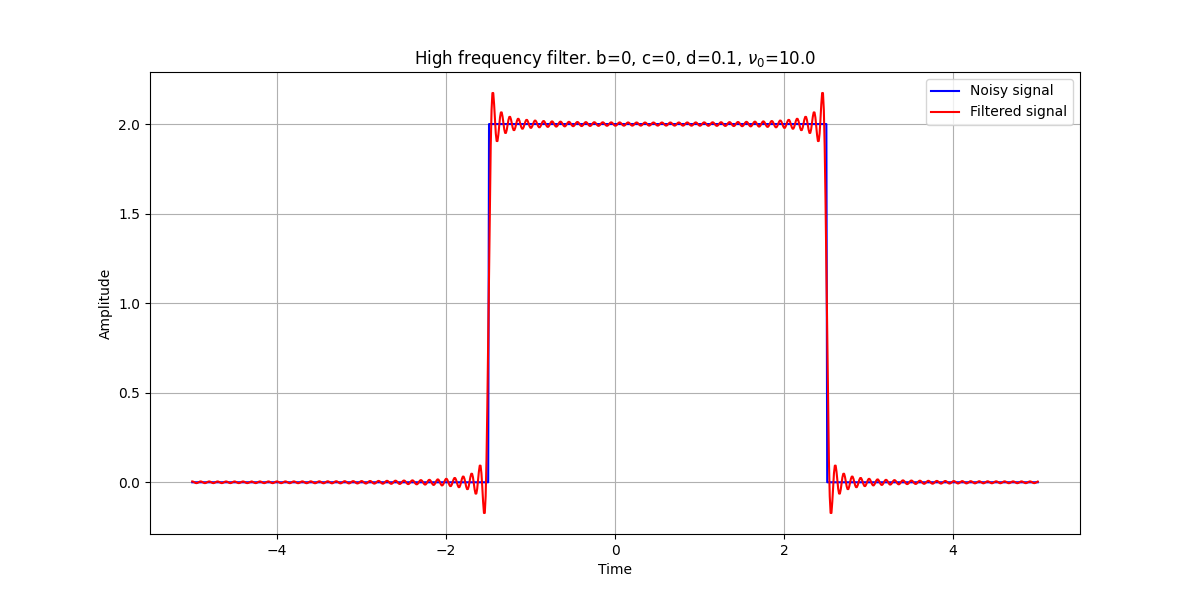
\includegraphics[scale=0.485]{4_u_flt_u_nohigh.png}
        \captionsetup{skip=0pt}
        \caption{График исходного и фильтрованного сигналов}
        \label{fig:fig9}
    \end{figure}
    \begin{figure}[!htb]
        \centering
        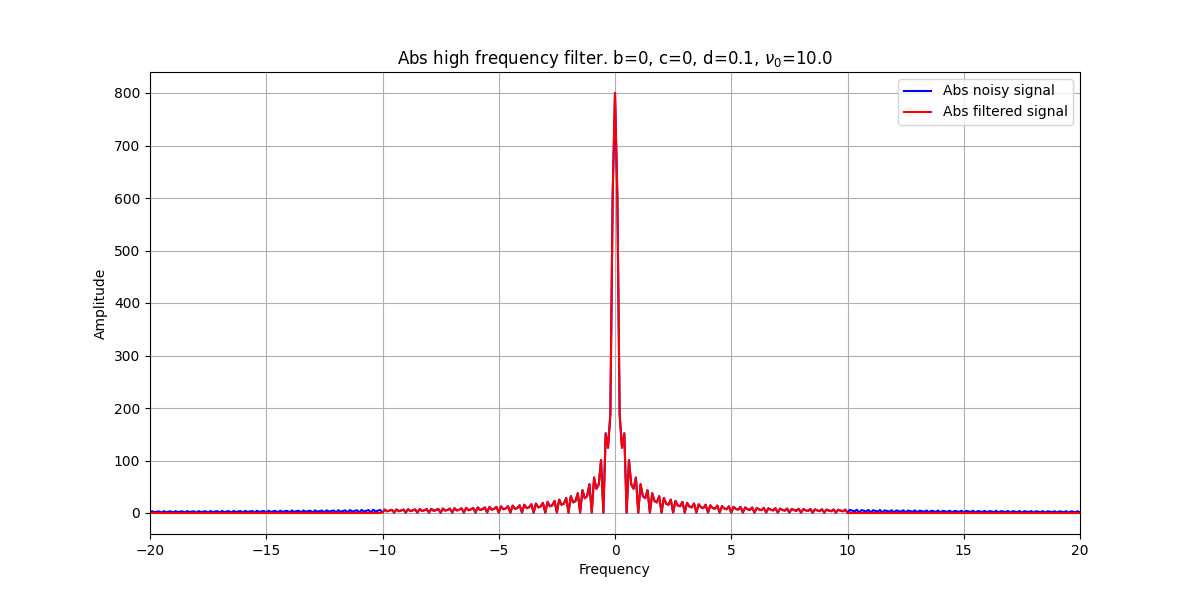
\includegraphics[scale=0.485]{4_abs_u_U_nohigh.png}
        \captionsetup{skip=0pt}
        \caption{График модуля Фурье-образа исходного и фильтрованного сигналов}
        \label{fig:fig10}
    \end{figure}
    \newpage
    \begin{figure}[!htb]
        \centering
        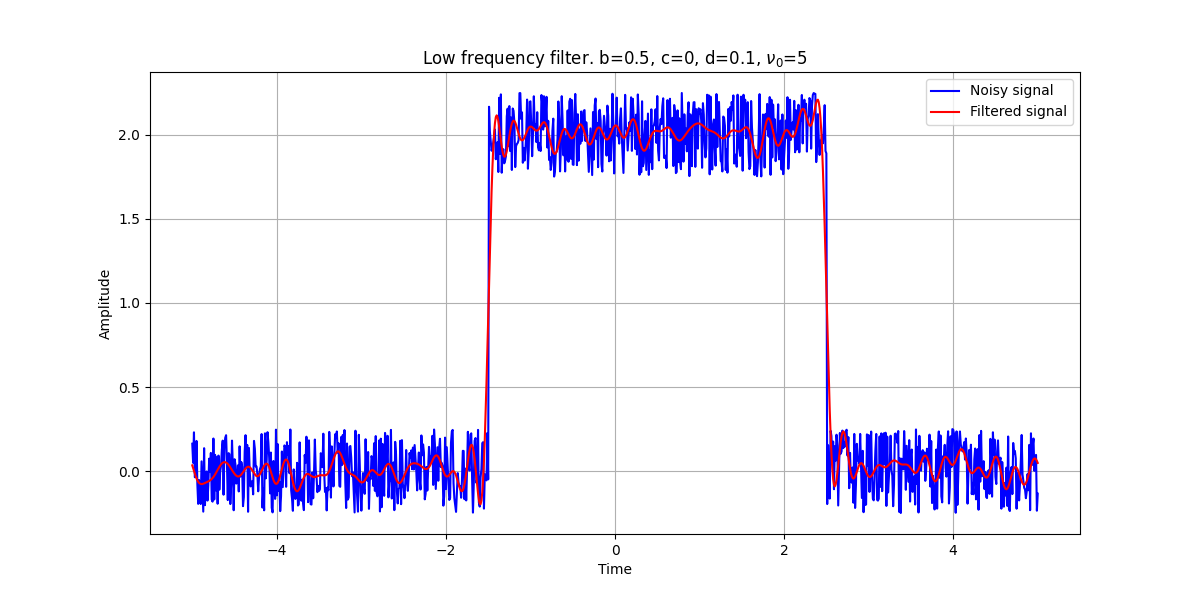
\includegraphics[scale=0.485]{8_u_flt_u_nohigh.png}
        \captionsetup{skip=0pt}
        \caption{График исходного и фильтрованного сигналов}
        \label{fig:fig11}
    \end{figure}
    \begin{figure}[!htb]
        \centering
        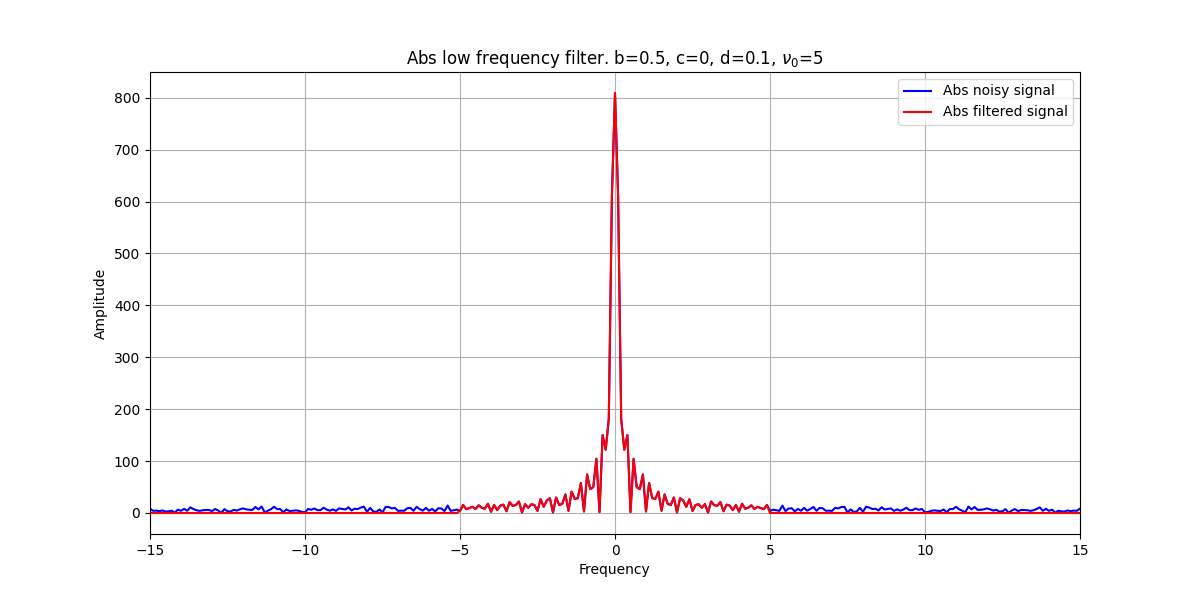
\includegraphics[scale=0.485]{8_abs_u_U_nohigh.png}
        \captionsetup{skip=0pt}
        \caption{График модуля Фурье-образа исходного и фильтрованного сигналов}
        \label{fig:fig12}
    \end{figure}
    \begin{figure}[!htb]
        \centering
        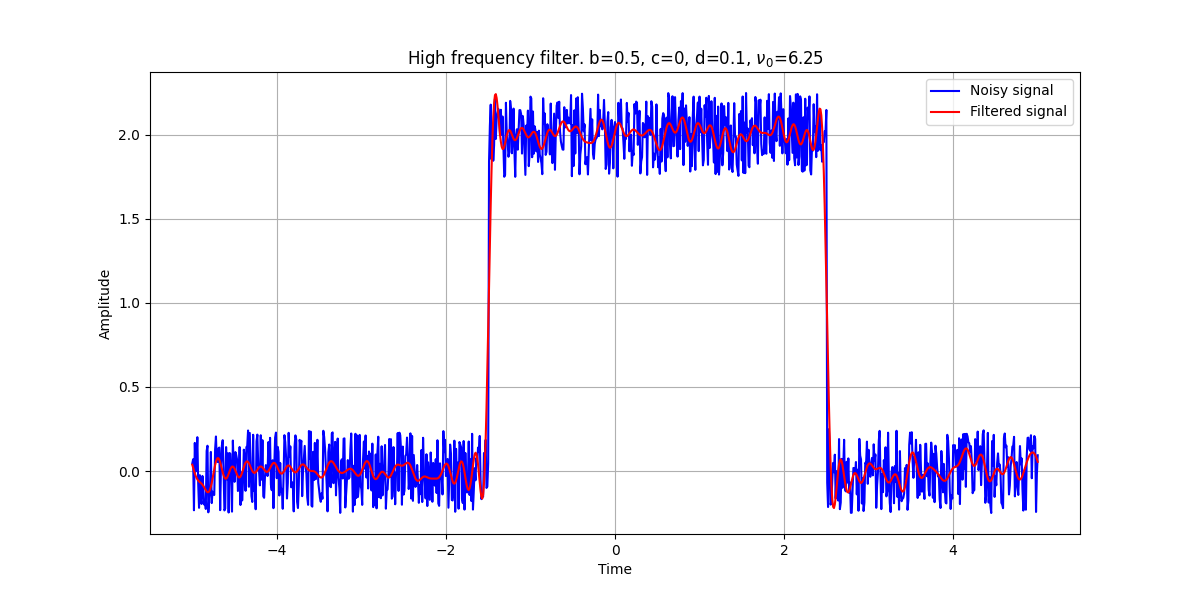
\includegraphics[scale=0.485]{7_u_flt_u_nohigh.png}
        \captionsetup{skip=0pt}
        \caption{График исходного и фильтрованного сигналов}
        \label{fig:fig13}
    \end{figure}
    \newpage
    \begin{figure}[!htb]
        \centering
        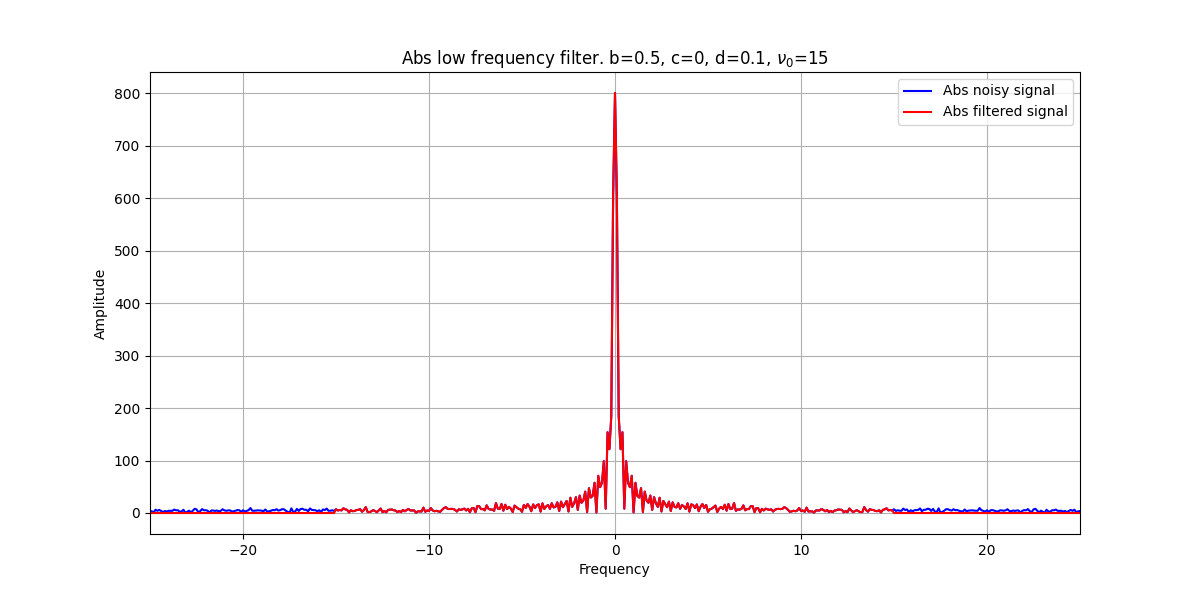
\includegraphics[scale=0.485]{7_abs_u_U_nohigh.png}
        \captionsetup{skip=0pt}
        \caption{График модуля Фурье-образа исходного и фильтрованного сигналов}
        \label{fig:fig14}
    \end{figure}
    \begin{figure}[!htb]
        \centering
        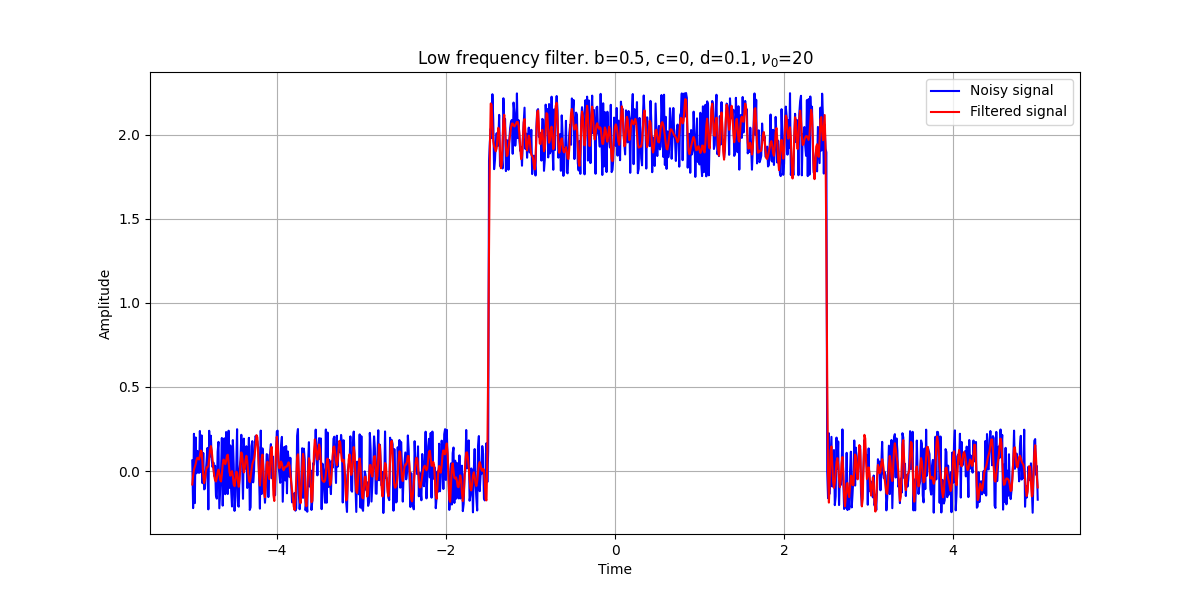
\includegraphics[scale=0.485]{6_u_flt_u_nohigh.png}
        \captionsetup{skip=0pt}
        \caption{График исходного и фильтрованного сигналов}
        \label{fig:fig15}
    \end{figure}
    \begin{figure}[!htb]
        \centering
        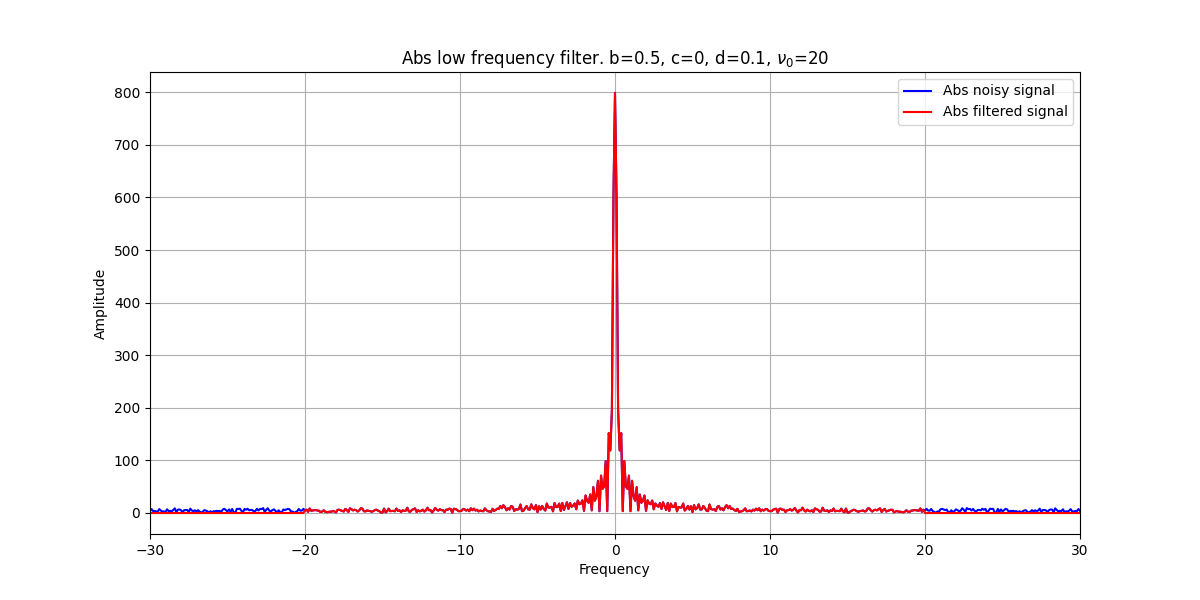
\includegraphics[scale=0.485]{6_abs_u_U_nohigh.png}
        \captionsetup{skip=0pt}
        \caption{График модуля Фурье-образа исходного и фильтрованного сигналов}
        \label{fig:fig16}
    \end{figure}
    \newpage
    \begin{figure}[!htb]
        \centering
        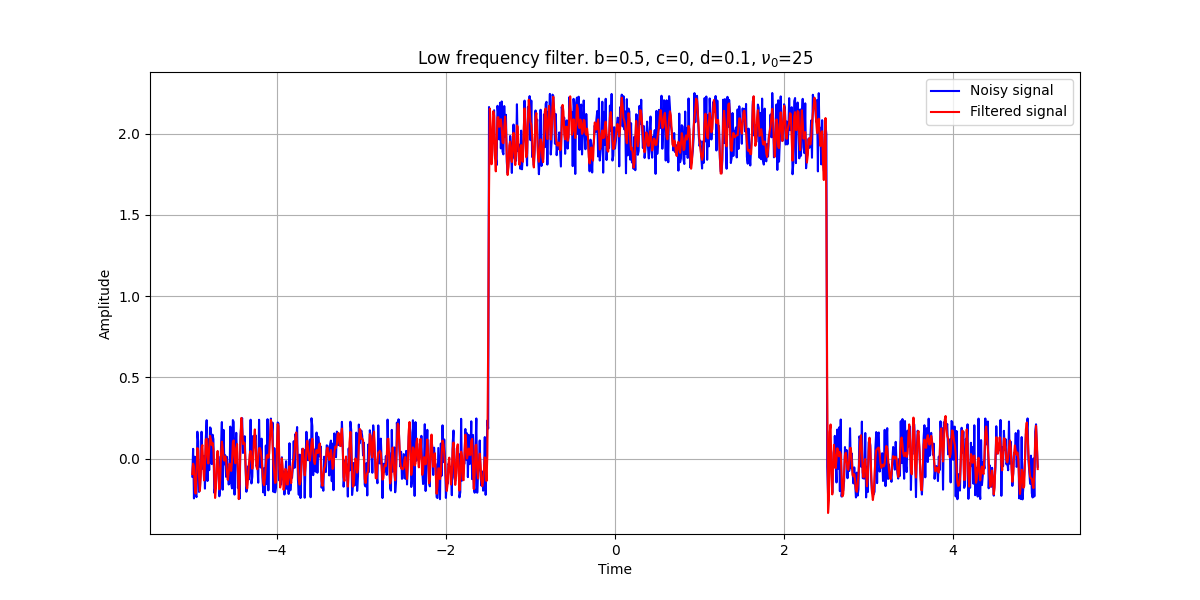
\includegraphics[scale=0.485]{10_u_flt_u_nohigh.png}
        \captionsetup{skip=0pt}
        \caption{График исходного и фильтрованного сигналов}
        \label{fig:fig17}
    \end{figure}
    \begin{figure}[!htb]
        \centering
        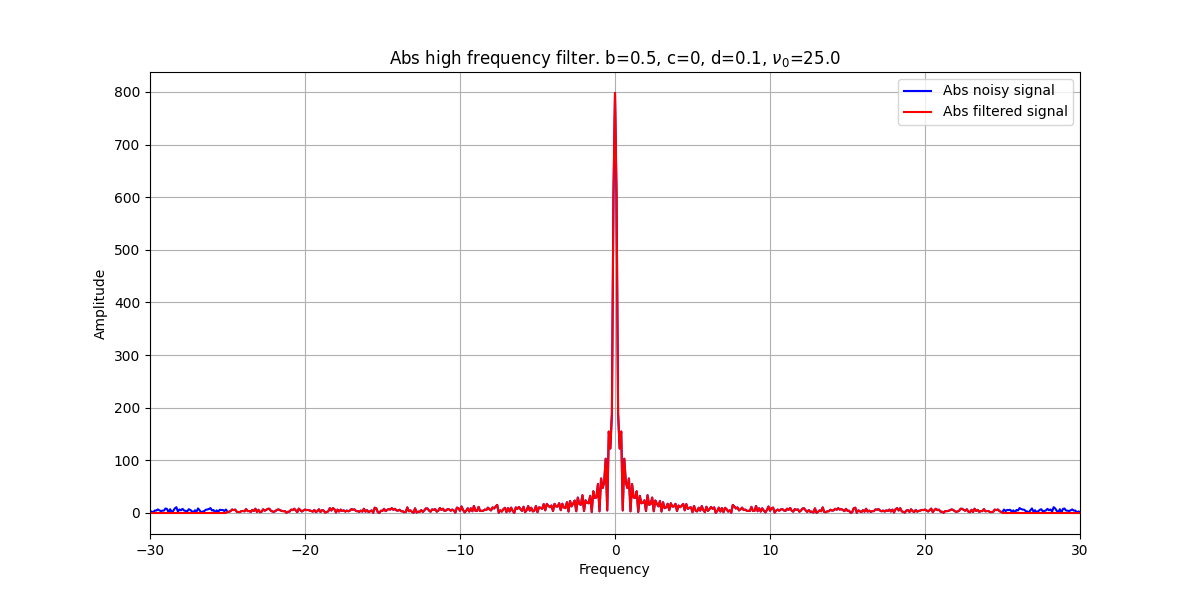
\includegraphics[scale=0.485]{10_abs_u_U_nohigh.png}
        \captionsetup{skip=0pt}
        \caption{График модуля Фурье-образа исходного и фильтрованного сигналов}
        \label{fig:fig18}
    \end{figure}
    \begin{figure}[!htb]
        \centering
        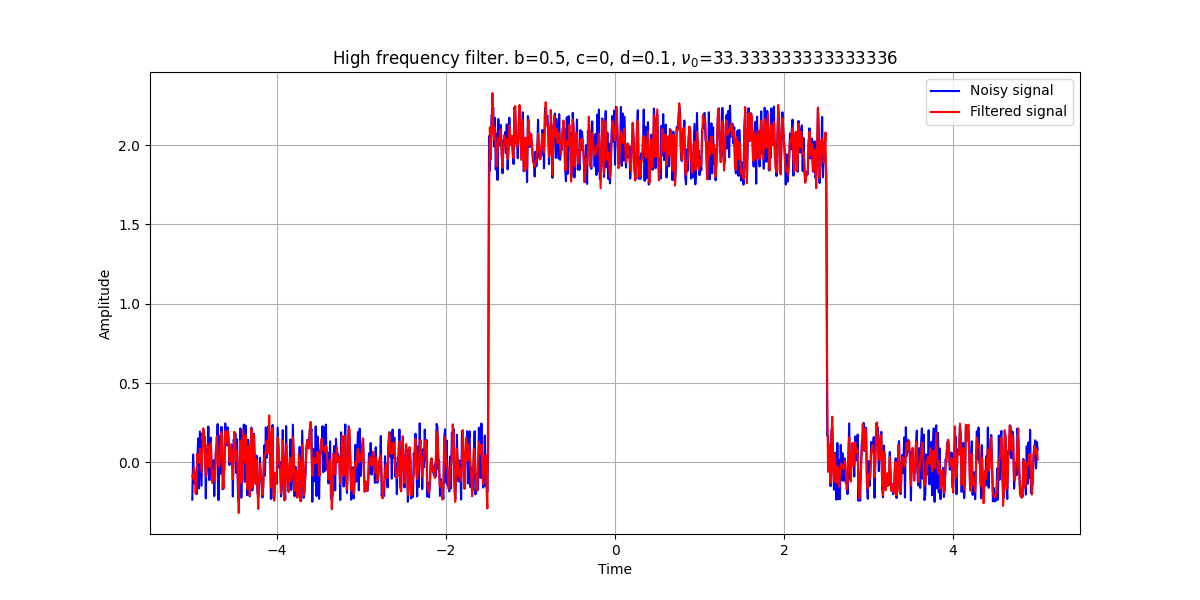
\includegraphics[scale=0.485]{9_u_flt_u_nohigh.png}
        \captionsetup{skip=0pt}
        \caption{График исходного и фильтрованного сигналов}
        \label{fig:fig19}
    \end{figure}
    \newpage
    \begin{figure}[!htb]
        \centering
        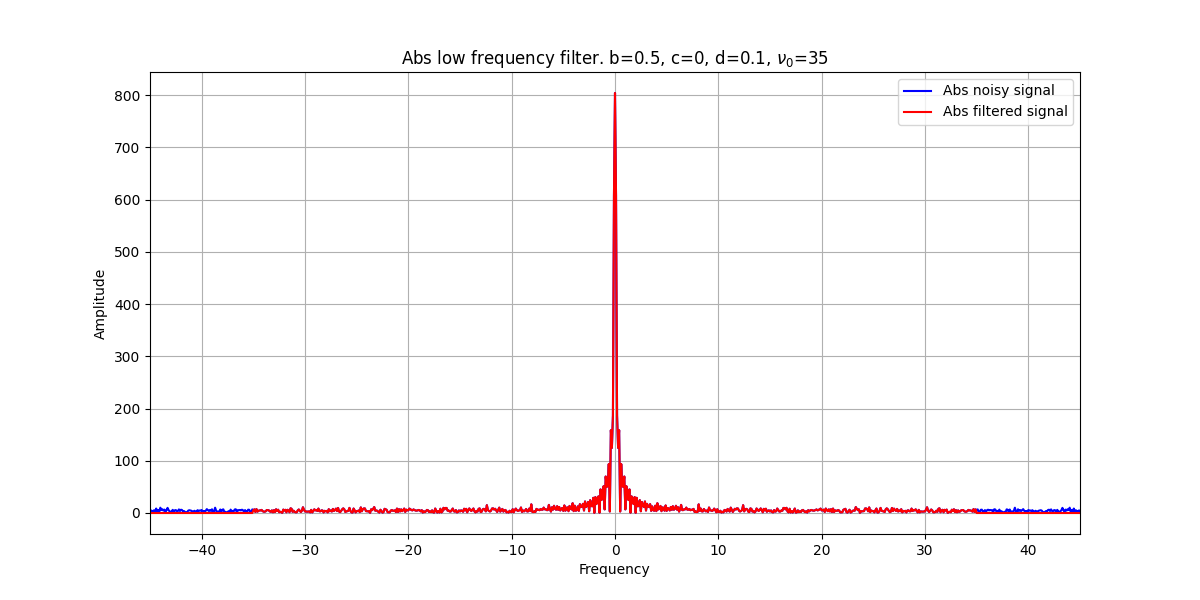
\includegraphics[scale=0.485]{9_abs_u_U_nohigh.png}
        \captionsetup{skip=0pt}
        \caption{График модуля Фурье-образа исходного и фильтрованного сигналов}
        \label{fig:fig20}
    \end{figure}
\end{document}